
%%
%%::::::::::::::::::::::::::::commands
\newcommand{\makeunderscorenormal}{\catcode`\_=8}
\newcommand{\makeunderscoreletter}{\catcode`\_=11}
\def\kw{%
    \begingroup
        \catcode`\_=11
%        \chardef\_=`\_  % not needed
        \kwset
    }
\def\kwset#1{%
        \ttfamily
        #1%
    \endgroup
    }
\newcommand{\kor}{$|$}

\makeatletter
\def\boxedminipage{\@ifnextchar [{\@iboxedminipage}{\@iboxedminipage[c]}}

\def\@iboxedminipage[#1]#2{\leavevmode \@pboxswfalse
  \if #1b\vbox
    \else \if #1t\vtop
             \else \ifmmode \vcenter
                       \else \@pboxswtrue $\vcenter
                    \fi
          \fi
  \fi\bgroup % start of outermost vbox/vtop/vcenter
    \hsize #2
    \hrule\@height\fboxrule
    \hbox\bgroup % inner hbox
      \vrule\@width\fboxrule \hskip\fboxsep \vbox\bgroup % innermost vbox
        \vskip\fboxsep
        \advance\hsize -2\fboxrule \advance\hsize-2\fboxsep
        \textwidth\hsize \columnwidth\hsize
        \@parboxrestore
        \def\@mpfn{mpfootnote}\def\thempfn{\thempfootnote}\c@mpfootnote\z@
        \let\@footnotetext\@mpfootnotetext
        \let\@listdepth\@mplistdepth \@mplistdepth\z@
        \@minipagerestore\@minipagetrue
        \everypar{\global\@minipagefalse\everypar{}}}

\def\endboxedminipage{%
        \par\vskip-\lastskip
        \ifvoid\@mpfootins\else
          \vskip\skip\@mpfootins\footnoterule\unvbox\@mpfootins\fi
        \vskip\fboxsep
      \egroup % ends the innermost \vbox
      \hskip\fboxsep \vrule\@width\fboxrule
    \egroup % ends the \hbox
    \hrule\@height\fboxrule
  \egroup% ends the vbox/vtop/vcenter
  \if@pboxsw $\fi}
\makeatother


% font
%\usepackage{helvet}
%\renewcommand{\familydefault}{\sfdefault}
% sectioning
%\makeatletter

\newcommand{\subpart}[1]{%
  \vspace{2\parskip}%
  \textbf{#1}%
  \hspace*{1em}%
}
\newcommand{\subsubpart}[1]{%
  \vspace{2\parskip}%
  \textit{#1}%
  \hspace*{1em}%
}
\newcommand{\subitempart}[2][$\bullet$]{%
  \vspace{2\parskip}%
  #1\hspace{1.em}\textbf{#2}\hspace{1.em}%
}
\newcommand{\subsubitempart}[2][--]{%
  \vspace{2\parskip}%
  #1\hspace{1.em}\textit{#2}\hspace{1.em}%
}
\newcommand{\note}[2][]{%
  \textit{#2}\hspace*{1em}
}
\makeatletter
\newcommand\subxsection{\@startsection{subsection}{2}{\z@}%
                                     {-3.25ex\@plus -1ex \@minus -.2ex}%
                                     {1.5ex \@plus .2ex}%
                                     {\normalfont\large\bfseries}}
\makeatother
%\makeatother
% miscellaneous
\newenvironment{inframe}{%
\noindent
\begin{lrbox}{\setbox1}
\begin{minipage}{\linewidth}%
}{%
\end{minipage}
\end{lrbox}
\framebox{\usebox{\box1}}
}
% foot note with choice of symbol 
\long\def\symbolfootnote[#1]#2{\begingroup%
\def\thefootnote{\fnsymbol{footnote}}\footnote[#1]{#2}\endgroup}
\long\def\symbolfootnotetext[#1]#2{\begingroup%
\def\thefootnote{\fnsymbol{footnote}}\footnotetext[#1]{#2}\endgroup}
% convenience
\newcommand{\ger}[1]{\emph{#1}}
\newcommand{\lat}[1]{#1}
\newcommand{\ie}{i.e.\@}
\newcommand{\cf}{cf.\@}
\newcommand{\eg}{e.g.\@}
\newcommand{\etal}{et al.\@}
\newcommand{\intro}[1]{\emph{#1}}
\newcommand{\fail}[1]{\emph{#1}}
%\newcommand{\tc}[1]{\ovalfbox{\textsf{#1}}}
\newcommand{\tc}[1]{%
\ifmmode
  \mathchoice{
    \ovalfbox{\textsf{\text{$#1$}}}
  }{
    \ovalfbox{\textsf{\text{$#1$}}}
  }{
    \ovalfbox{\textsf{\text{$\scriptstyle #1$}}}
  }{
    \ovalfbox{\textsf{\text{$\scriptscriptstyle #1$}}}
  }
\else
\ovalfbox{\textsf{#1}}%
\fi}
\newcommand{\name}[1]{#1}
% rotate
\newcommand{\textrotl}[1]{%
\setbox2=\hbox{#1}
\rotl2
}
% source code style
\newcommand{\cod}[1]{\texttt{\textup{#1}}}
\newenvironment{codenv}{\begin{quote} \tt}{\end{quote}}
\newcommand{\cor}{$|$}
\newcommand{\cgb}{$($}
\newcommand{\cge}{$)$}
\newcommand{\ccb}{$[$}
\newcommand{\cce}{$]$}
\newcommand{\cnl}{} %%$\setminus$}
\newcommand{\chs}{\hspace{3em}}


% bold Figure 7.5 at figures
\makeatletter
\long\def\@makecaption#1#2{%
  \vskip-0.65\abovecaptionskip
  \sbox\@tempboxa{\textbf{#1:} #2}%
  \ifdim \wd\@tempboxa >\hsize
    \textbf{#1:} #2\par
  \else
    \global \@minipagefalse
    \hb@xt@\hsize{\hfil\box\@tempboxa\hfil}%
  \fi
  \vskip\belowcaptionskip}
\makeatother
%%% Local Variables: 
%%% mode: latex
%%% TeX-master: "inventory"
%%% End: 

%% mathematical abbreviations
%%\usepackage{helvet}
%%\renewcommand{\familydefault}{\sfdefault}
%\usepackage{amsmath,amssymb,color}  % and more

% extra colourful stuff
%%\newcommand{\mathbl}[1]{\text{\textcolor[rgb]{0.0,0.0,0.69}{$#1$}}}
%\newcommand{\mathbl}[1]{#1}
%%\newcommand{\mathgr}[1]{\text{\textcolor[rgb]{0.0,0.69,0.0}{$#1$}}}
%\newcommand{\mathgr}[1]{#1}

%% mathematical operators
\newcommand{\ii}{\mathrm{i}}  % complex i
\newcommand{\dd}{\mathrm{d}}  % differential d
\newcommand{\pd}{\partial}  % partial differentiation d
\newcommand{\DD}{\mathrm{D}}  % linearisation operator
\newcommand{\Alpha}{\mathcal{A}}
\newcommand{\levicivita}{\mathcal{E}}  % Levi-Civita symbol
%\newcommand{\tns}[1]{\underline{\boldsymbol{#1}}}  % tensor
%\newcommand{\tnsfour}[1]{\mathsf{#1}}
\newcommand{\tns}[2][0]{
\def\myinput{#2}
% \count0=#1
% \ifnum\count0=1
%   \def\myinput{#2}
% \fi
% \ifnum\count0=2
%   \def\myinput{#2}
% \fi
% \ifnum\count0=4
%   \def\myinput{\tnsfour{#2}}
% \fi
\dimen1=0.5pt  % truncation length of underline
\mathchoice{
  \setbox0=\hbox{$\boldsymbol{\myinput{}}$}
  \dimen2=\wd0
  \ifdim\dimen2>\dimen1
    \advance\dimen2 by -2\dimen1
  \fi
  \wd0=\dimen2
  \setbox1=\hbox{\hskip\dimen1\underline{\hskip-\dimen1\box0}\hskip2\dimen1}
  \box1
}{
  \setbox0=\hbox{$\boldsymbol{\textstyle \myinput{}}$}
  \dimen2=\wd0
  \ifdim\dimen2>\dimen1
   \advance\dimen2 by -2\dimen1
  \fi
  \wd0=\dimen2
  \setbox1=\hbox{\hskip\dimen1\underline{\hskip-\dimen1\box0}\hskip2\dimen1}
  \box1
}{
  \setbox0=\hbox{$\boldsymbol{\scriptstyle \myinput{}}$}
  \dimen2=\wd0
  \ifdim\dimen2>\dimen1
    \advance\dimen2 by -2\dimen1
  \fi
  \wd0=\dimen2
  \setbox1=\hbox{\hskip\dimen1\underline{\hskip-\dimen1\box0}\hskip2\dimen1}
  \box1
}{
  \setbox0=\hbox{$\boldsymbol{\scriptscriptstyle \myinput{}}$}
  \dimen2=\wd0
  \ifdim\dimen2>\dimen1
    \advance\dimen2 by -2\dimen1
  \fi
  \wd0=\dimen2
  \setbox1=\hbox{\hskip\dimen1\underline{\hskip-\dimen1\box0}\hskip2\dimen1}
  \box1
}}
\newcommand{\hattns}[1]{\hat{\tns{#1}}}  % tensor with hat
\newcommand{\dottns}[1]{\dot{\tns{#1}}}  % tensor with dot
\newcommand{\bartns}[1]{\bar{\tns{#1}}}  % tensor with bar
\newcommand{\bretns}[1]{\breve{\tns{#1}}}  % tensor with breve
\newcommand{\chetns}[1]{\check{\tns{#1}}}  % tensor with check
\newcommand{\tiltns}[1]{\tilde{\tns{#1}}}  % tensor with tilde
\newcommand{\ddottns}[1]{\ddot{\tns{#1}}}  % tensor with to dots
\newcommand{\mat}[1]{\boldsymbol{#1}}  % matrix
\newcommand{\barmat}[1]{\bar{\mat{#1}}}  % matrix with bar
\newcommand{\vct}[1]{\boldsymbol{#1}}  % vector
\newcommand{\hatvct}[1]{\hat{\vct{#1}}}  % vector with hat
\newcommand{\hatdotvct}[1]{\hat{\dotvct{#1}}}  % vector with hat and dot
\newcommand{\dotvct}[1]{\dot{\vct{#1}}}  % vector with dot
\newcommand{\ddotvct}[1]{\ddot{\vct{#1}}}  % vector with double dots
\newcommand{\dddotvct}[1]{\dddot{\vct{#1}}}  % vector with triple dots
\newcommand{\barvct}[1]{\bar{\vct{#1}}}  % vector with bar
\newcommand{\tildevct}[1]{\tilde{\vct{#1}}}  % vector with tilde
\newcommand{\tilvct}[1]{\tilde{\vct{#1}}}  % vector with tilde
\newcommand{\chevct}[1]{\check{\vct{#1}}}  % vector with check
\newcommand{\T}{\mathrm{T}}  % transpose T
\newcommand{\bre}[1]{\breve{#1}}  % short for breve
\newcommand{\che}[1]{\check{#1}}  % short for check
\newcommand{\adiag}[1]{\overset{\scriptscriptstyle\smallsetminus}{#1}}
\newcommand{\alowtri}[1]{\overset{\scriptscriptstyle\llcorner}{#1}}
\newcommand{\grad}{\mathrm{grad}}  % (spatial) gradient
\newcommand{\Grad}{\mathrm{Grad}}  % (material) gradient
\newcommand{\ddiv}{\mathrm{div}}  % divergence in spatial frame
\newcommand{\Ddiv}{\mathrm{Div}}  % divergence in material frame
\newcommand{\dirac}{\delta}  % Dirac's delta
\newcommand{\cof}{\mathrm{cof}}  % (spatial) gradient
\newcommand{\forwhich}{\;|\;}
% \newcommand{\ass}[3][d]{%  % assembly operator, 'd' display style, 't' text style
% \if#1d
% \overset{#3}{\underset{#2}{\raisebox{-0.6ex}{\mbox{\huge $\mathsf{A}$}}}}
% \else
% \raisebox{-0.4ex}{\mbox{\Large $\mathsf{A}$}}_{#2}^{#3}
% \fi
% }
\newcommand{\Ass}[3][d]{%  % assembly operator
% option 'd' is useless
\mathchoice{  % display style
\overset{#3}{\underset{#2}{\raisebox{-0.6ex}{\mbox{\huge $\mathsf{A}$}}}}
}{  % text style
\raisebox{-0.35ex}{\mbox{\Large $\mathsf{A}$}}_{#2}^{#3}
}{  % script style
\raisebox{-0.35ex}{\mbox{\Large $\mathsf{A}$}}_{#2}^{#3}
}{  % scriptscript style
\raisebox{-0.35ex}{\mbox{\Large $\mathsf{A}$}}_{#2}^{#3}
}}

\newcommand{\loc}{\mathrm{loc}}  % location mapping
\newcommand{\stat}{\mathrm{stat}}  % location mapping
\newcommand{\domainsum}{\bigcup}
\newcommand{\abs}[1]{|#1|}
\newcommand{\Abs}[1]{\|#1\|}
% \ifmmode ... \else ... \fi
\newcommand{\Nabla}{\nabla_{\!0}}
\newcommand{\incr}{\Delta}
\newcommand{\Lin}{\mathrm{Lin}}  % linearisation
\newcommand{\trace}{\mathrm{tr}}  % trace of quadratic tensor

%% symbols
\newcommand{\eps}{\varepsilon}  % epsilon
\newcommand{\sig}{\sigma}  % epsilon
\newcommand{\const}{\mathrm{const}}  % constant
\newcommand{\R}{\mathbb{R}}  % real set of numbers R
\newcommand{\CC}{\mathbb{C}}  % complex set of numbers C
\newcommand{\ndof}{\mathit{ndof}}  % number of degrees of freedom
\newcommand{\nnod}{\mathit{nnod}}  % number of nodes
\newcommand{\nele}{\mathit{nele}}  % number of elements
\newcommand{\eenh}{\mathit{eenh}}  % number of element enhancements
\newcommand{\enod}{\mathit{enod}}  % number of element nodes
\newcommand{\numgp}{\mathit{numgp}}  % number of Gausspoints in direction 
\newcommand{\nco}{\mathit{nco}}  % number of active contact sets 
\newcommand{\BE}{\text{BE}}  % balance equations
\newcommand{\FBC}{\text{FBC}}  % flux boundary conditions
\newcommand{\DBC}{\text{DBC}}  % Dirichlet boundary conditions
\newcommand{\TPE}{\text{TPE}}  % total potential energy
\newcommand{\EEE}{\text{EE}}  % strain-strain connection
\newcommand{\SSS}{\text{SS}}  % stress-stress connection
\newcommand{\FFF}{\text{FF}}  % defgrad-defgard connection
\newcommand{\PPP}{\text{PP}}  % 1PK-1PK stress connection 
\newcommand{\HR}{\text{HR}}  % Hellinger--Reissner
\newcommand{\HW}{\text{HW}}  % Hu--Washizu
\newcommand{\Int}{\text{int}}  % internal
\newcommand{\Ext}{\text{ext}}  % external
\newcommand{\HOT}{\mathit{HOT}}  % higher order terms
\newcommand{\Dt}{\Delta t}  % time step size
\newcommand{\effdyn}{\text{effdyn}}  % effective dynamic
\newcommand{\Teffdyn}{\text{Teffdyn}}  % effective dynamic
\newcommand{\PK}{\text{PK2}}  % 2nd Piola--Kirchhoff
\newcommand{\Pk}{\text{PK1}}  % 1st Piola--Kirchhoff
\newcommand{\KI}{\text{K}}  % Kirchhoff
\newcommand{\GL}{\text{GL}}  % Green--Lagrange
\newcommand{\EA}{\text{E}}  % Euler--Almansi
\newcommand{\Eng}{\text{i}}  % engineering
\newcommand{\Nat}{\text{n}}  % natural / logarithmic
\newcommand{\TSO}{\textrm{II}}  % theory of second order
\newcommand{\TFO}{\textrm{I}} % theory of 1st order
\newcommand{\CT}{\text{C}}  % Cauchy / true
\newcommand{\BI}{\text{B}}  % Biot
\newcommand{\VK}{\text{VK}}  % St. Venant-Kirchhoff
\newcommand{\Tang}{\text{T}}  % tangential
\newcommand{\ela}{\text{e}}  % elastic
\newcommand{\geo}{\text{g}}  % geometric
\newcommand{\ini}{\text{u}}  % initial
\newcommand{\loa}{\text{L}}  % load
\newcommand{\tol}{\mathit{tol}}  % tolerance
\newcommand{\LL}{\text{L}}  % `linear'
\newcommand{\enh}{\mathit{enh}}  % enhanced
\newcommand{\red}{\text{red}}  % reduced
\newcommand{\crit}{\text{crit}}  % critical
\newcommand{\Inva}{I}
\newcommand{\INva}{I\!\!I}
\newcommand{\INVa}{I\!\!I\!\!I}
\newcommand{\Mat}{\text{m}}


%% convenience
\newcommand{\unit}[1]{\,\mathrm{#1}}  % unit
\newcommand{\EE}[1]{\cdot 10^{#1}}  % "scientific notation" for 10 to the power of 
\newcommand{\virt}{\delta}  % variation of first kind / virtual
\newcommand{\set}[1]{\mathcal{#1}}  % set
\newcommand{\script}[1]{\mathcal{#1}}

%% text font stuff
\newcommand{\period}{\text{.}}
\newcommand{\comma}{\text{,}}
%\newcommand{\colon}{\text{:}}
\newcommand{\semicolon}{\text{;}}

%% circled text (EgyptTeX)
%%\newcommand{\tc}[1]{%
%%\ifmmode
%%  \mathchoice{
%%    \ovalfbox{\textsf{\text{$#1$}}}
%%  }{
%%    \ovalfbox{\textsf{\text{$#1$}}}
%%  }{
%%    \ovalfbox{\textsf{\text{$\scriptstyle #1$}}}
%%  }{
%%    \ovalfbox{\textsf{\text{$\scriptscriptstyle #1$}}}
%%  }
%%\else
%%\ovalfbox{\textsf{#1}}%
%%\fi}

%% special
\newcommand{\sboxed}[1]{\boxed{\scriptstyle#1}}
\newcommand{\Underline}[1]{\underline{\underline{#1}}}  % double underline
\newcommand{\underneath}[3][0pt]{  % place text underneath symbol
\setbox0=\hbox{$|$}
\dimen2=\ht0
\advance\dimen2 by #1
\setbox0=\hbox{\vrule height\dimen2}
\setbox1=\hbox{$\displaystyle #2$}
\setbox5=\hbox{$#3$}
\dimen5=\dp5
\advance\dimen5 by 2pt
\setbox2=\hbox{\vrule width0pt height\ht5 depth\dimen5 \box5}
\dimen0=\dp0
\advance\dimen0 by \ht2
\advance\dimen0 by 2pt
\dimen1=0.5\wd1
\ifdim\wd1>\wd2
\dimen4=0.5\wd2
\else
\dimen4=0.5\wd1
\fi
\setbox3=\hbox{\copy0\hskip-\dimen4\lower\dimen0\copy2}
\dimen3=\ht3
\advance\dimen3 by \dp1
\advance\dimen3 by 2pt
\setbox4=\hbox to \wd1 {\copy1\hskip-\dimen1\lower\dimen3\copy3}
\box4
}
\newcommand{\overneath}[3][0pt]{  % place text underneath symbol
\setbox0=\hbox{$|$}
\dimen2=\ht0
\advance\dimen2 by #1
\setbox0=\hbox{\vrule height\dimen2}
\setbox1=\hbox{$\displaystyle #2$}
\setbox2=\hbox{$#3$}
\dimen0=\ht0
\advance\dimen0 by \dp2
\advance\dimen0 by 2pt
\dimen1=0.5\wd1
\ifdim\wd1>\wd2
\dimen4=0.5\wd2
\else
\dimen4=0.5\wd1
\fi
\setbox3=\hbox{\copy0\hskip-\dimen4\raise\dimen0\copy2}
\dimen3=\ht1
%\advance\dimen3 by \ht1
\advance\dimen3 by 2pt
\setbox4=\hbox to \wd1 {\copy1\hskip-\dimen1\raise\dimen3\copy3}
\box4
}
%%
%%
\makeatletter
\newcommand{\strikethrough}[2][d]{%
\unitlength=1pt%
\newcount\extraspace
\extraspace=5
\newbox\arg%
% switch to (displayed) math mode
\ifmmode  % switch to (displayed) math mode or text mode
\if#1d  % switch to display style if 'd' option
\setbox\arg=\hbox{$\displaystyle #2$}%
\else  % switch to text style  if 't' option
\setbox\arg=\hbox{$\textstyle #2$}%
\fi
\else
\setbox\arg=\hbox{#2}%
\fi
% get argdepth
\newcount\argdepth%
\setbox1=\hbox{%
\global\argdepth=\strip@pt\dp\arg
\global\advance\argdepth by \the\extraspace
}%
% get argheight
\newcount\argheight%
\setbox1=\hbox{%
\global\argheight=\strip@pt\ht\arg
\global\advance \argheight by \the\argdepth
%\global\advance \argheight by \the\extraspace
}%
% get argwidth
\newcount\argwidth%
\setbox1=\hbox{%
\global\argwidth=\strip@pt\wd\arg
\global\advance\argwidth by \the\extraspace
\global\advance\argwidth by \the\extraspace
}%
% create output box
\newbox\product%
\setbox\product=\hbox{%
\begin{picture}(\the\argwidth,\the\argheight)
% draw a nice box (debug purposes)
%\put(0,-\the\argdepth){\line(1,0){\the\argwidth}}
%\put(0,-\the\argdepth){\line(0,1){\the\argheight}}
%\put(0,-\the\argdepth){\line(0,1){\the\argheight}}
%\put(0,\strip@pt\ht\arg){\line(1,0){\the\argwidth}}
\qbezier(0,-\the\argdepth)(0,-\the\argdepth)(\the\argwidth,\the\argheight)
%\put(\the\argwidth,\the\argheight){tip}  % debug purposes
\put(\the\extraspace,0){\box\arg}
\end{picture}}%
\box\product%
}
\makeatother

%%% Local Variables: 
%%% mode: plain-tex
%%% TeX-master: "fe"
%%% End: 


%%
%%::::::::::::::::::::::::::::dynamics
\chapter{Structural dynamics}\label{struct_dynamics:chap}

%% This documents should be split to several files which describe the
%% individual time integration schemes. Right now, we do not have readily
%% available theoretical background information.

\section{Input parameters}

\subsection{Common parameters}
\begin{verbatim}
------------------------------------------------STRUCTURAL DYNAMIC
\end{verbatim}

\kw{DYNAMICTYP} $string$\\
type of time integration control with method $string$, i.e.\\
\begin{tabular}{lll}
   $string$ & meaning & valid with
\\ \kw{Gen_Alfa} & generalized-alpha & \ccarat{}, \baci{} \texttt{StruGenAlpha}
\\ \kw{Centr_Diff} & central differences & \ccarat{}
\\ \kw{Gen_EMM} & generalized energy-momentum method & \ccarat{}
\\ \kw{Static} & static analysis & \baci{} \texttt{StruGenAlpha}
\\ \kw{GenAlpha} & generalised energy-momentum method & \baci{} \texttt{STR::TimInt}
\\ \kw{OneStepTheta} & one-step-theta method & \baci{} \texttt{STR::TimInt}
\\ \kw{GEMM} & generalised energy-momentum method & \baci{} \texttt{STR::TimInt}
\\ \kw{Statics} & static analysis & \baci{} \texttt{STR::TimInt}
\\ \kw{AdamsBashforth2} & Adams-Bashforthn 2nd order & \baci{} \texttt{STR::TimInt}
\end{tabular}

\kw{EIGEN} (\kw{1}\kor\kw{0})\\
EIGEN make eigenanalysis of the initial dynamic system (not with every solver): (0,1)\\
\textbf{Remark:} Does not work anywhere.

\kw{RESEVRYDISP} $int$\\
save displacements and contact forces every $int$ steps

\kw{RESEVRYSTRS} $int$\\
save stresses every $int$ steps

\kw{RESTARTEVRY} $int$\\
write restart possibility to .pss every $int$ steps

\kw{TIMESTEP} $real$\\
time step size

\kw{NUMSTEP} $int$\\
maximum number of steps

\kw{MAXTIME} $real$\\
maximum time

\kw{DAMPING} $string$\\
\begin{tabular}{lll}
   $string$ & meaning & valid in
\\ \kw{No} & no global damping & \ccarat{}, \baci{}
\\ \kw{Yes} & Rayleigh-damping & \ccarat{}, \baci{}
\\ \kw{Rayleigh} & Rayleigh-damping & \baci{}
\\ \kw{Material} & material-based damping on element-level & \baci{}
\end{tabular}


\kw{M_DAMP} $real$\\
Rayleigh-coefficient for Rayleigh damping proportional to mass matrix $\text{M\_DAMP} \times M$

\kw{K_DAMP} $real$\\
Rayleigh-coefficient for Rayleigh damping proportional to initial/reference stiffness matrix $\text{K\_DAMP} \times K$

\kw{NLNSOL} $string$\\
type of non-linear solution technique chosen, i.e.\\
\begin{tabular}{lll}
   $string$ & meaning & valid with
\\ \kw{fullnewton} & full Newton-Raphson iteration  (tangential) & \ccarat{}, \baci{}
\\ \kw{modnewton} & modified Newton-Raphson iteration (secantial) & \ccarat{}, \baci{}
\\ \kw{matfreenewton} & matrix-free Newton-Raphson iteration & \ccarat{}, \baci{}
\\ \kw{nlncg} & non-linear conjugate-gradient method & \ccarat{}, \baci{}
\\ \kw{ptc} & ??? & \ccarat{}, \baci{} \texttt{StruGenAlpha}
\\ \kw{lsnewton} & line-search Newton & \baci{} \texttt{StruGenAlpha}
\\ \kw{newtonlinuzawa} & linearised Newton-Uzawa & \baci{}
\\ \kw{augmentedlagrange} & non-linear Newton-Uzawa & \baci{}
\end{tabular}

\kw{TOLDISP} $real$\\
tolerance in the displacement norm for the Newton iteration 

\kw{MAXITER} $int$\\
maximum number of iterations allowed for newton iteration before failure

\subsection{\ccarat{} parameters}

\kw{ITERATION} (\kw{mod}\kor\kw{full}\kor\kw{none})\\
make Newton Iteration (only full implemented, ignored by explicit
time int.)

\kw{BETA} $real$\\
\kw{GAMMA} $real$\\
\kw{ALPHA_M} $real$\\
\kw{ALPHA_F} $real$\\
\kw{BETA}, \kw{GAMMA}, \kw{ALPHA_M} and \kw{ALPHA_F} generalized-$\alpha$
factors, \kw{BETA} and \kw{GAMMA} also 
used by explicit time integration

\kw{XSI} $real$\\
disspipation parameter for GEMM time integration

\kw{CONTACT} (\kw{Yes}\kor\kw{No})\\
switch contact algorithms for shell8 and wall1 on/off;
Have to use \kw{SPOOLES_nonsym} in parallel as solver for contact problems

\kw{CET_flag} (\kw{Yes}\kor\kw{No})\\
switch enforcement for contact lagr. multipliers on/off;
\kw{Yes} $\to$ penalty method, \kw{No} $\to$ augmented Lagrangean

\kw{FR_flag} (\kw{Yes}\kor\kw{No})\\
switch friction in contact on/off: (0,1)

\kw{NPP} $real$\\
penaly parameter for normal contact

\kw{TPP} $real$\\
penaly parameter for tangential (frictional) contact

\kw{FR_COEF} $real$\\
frictional coefficient

\kw{TIMEADAPT} (\kw{Yes}\kor\kw{No})\\
switch time adaptivity dependend on number of newton iterations on/off (only shell8)

\kw{ITWANT} $int$\\
number of newton iterations wanted (adaptivity)

\kw{MAXDT} $real$\\
maximum time step size allowed to the time adaptivity

\kw{RESULTDT} $real$\\
offset when results shall be written to .flavia.res when time adaptivity is on

\subsection{\baci{} common parameters}

\kw{RESEVRYERGY} $int$\\
write system energies every requested $int$th step

\kw{TOLRES} $real$\\
tolerance in the residual forces norm for the Newton iteration (generalised-alpha)

\kw{TOLCONSTR} $real$\\
tolerance in the constraint error norm for the Newton iteration

\kw{CONV_CHECK} $string$\\
type of convergence check in non-linear solution technique, i.e. with respect to \kw{TOLDISP} and \kw{TOLRES} we have the following control possibilities\\
\begin{tabular}{lll}
   $string$ & meaning
\\ \kw{AbsRes_And_AbsDis} & absolute norm of residual forces AND absolute norm of iterative displacements increments \\
\\ \kw{AbsRes_Or_AbsDis} & absolute norm of residual forces OR absolute norm of iterative displacements increments
\\ \kw{RelRes_And_AbsDis} & relative norm of residual forces AND absolute norm of iterative displacements increments 
\\ \kw{RelRes_Or_AbsDis}  & relative norm of residual forces OR absolute norm of iterative displacements increments  
\\ \kw{RelRes_And_RelDis} & relative norm of residual forces AND relative norm of iterative displacements increments 
\\ \kw{RelRes_Or_RelDis} & relative norm of residual forces OR relative norm of iterative displacements increments  
\end{tabular}
The relative norms are calculated by dividing the absolute norm by the norm of the overall displacements and the maximum norm of internal, external, inertial (and possibly viscous) forces of the last time step, respectively.


\kw{ADAPTCONV} (\kw{No}\kor\kw{Yes})\\
Switch on adaptive control of linear solver tolerance for nonlinear solution

\kw{ADAPTCONV_BETTER} $float$\\
The linear solver shall be this much better than the current nonlinear residual in the nonlinear convergence limit

\kw{PREDICT} $string$\\
set predictor for non-linear solution technique
\begin{tabular}{ll}
   \kw{Vague} & undetermined
\\ \kw{ConstDis} & constant displacements, consistent velocities and accelerations
\\ \kw{ConstDisVelAcc} & consta displacements, velocties and accelerations
\end{tabular}

\kw{UZAWAPARAM} $float$\\
Parameter for Uzawa algorithm dealing with lagrange multipliers

\kw{UZAWATOL} $float$\\
Tolerance for iterative solve with Uzawa algorithm

\kw{UZAWAMAXITER} $int$\\
maximum number of iterations allowed for uzawa algorithm before failure going to next newton step

\kw{UZAWAALGO} (\kw{iterative}\kor\kw{direct})\\
Uzawa algorithm

\subsection{\baci{} \texttt{StruGenAlpha}  parameters}

\kw{BETA} $real$\\
$\beta$ factor of generalized-$\alpha$

\kw{GAMMA} $real$\\
$\gamma$ factor of generalized-$\alpha$

\kw{ALPHA_M} $real$\\
$\alpha_m$ factor of generalized-$\alpha$

\kw{ALPHA_F} $real$\\
$\alpha_f$ factor of generalized-$\alpha$

\subsection{\baci{} \texttt{STR::TimInt} parameters}

\begin{verbatim}
---------------------------------------STRUCTURAL DYNAMIC/GENALPHA
\end{verbatim}

\kw{GENAVG} (\kw{ImrLike}\kor\kw{TrLike})\\
mid-average type of internal forces

\kw{BETA} $real$\\
Generalised-alpha coefficient in $(0,1/2]$

\kw{GAMMA} $real$\\
Generalised-alpha factor in $(0,1]$

\kw{ALPHA_M} $real$\\
Generalised-alpha factor in $[0,1)$

\kw{ALPHA_F} $real$\\
Generalised-alpha factor in $[0,1)$

\begin{verbatim}
-----------------------------------STRUCTURAL DYNAMIC/ONESTEPTHETA
\end{verbatim}

\kw{THETA}
One-step-theta coefficient $\theta$ in $(0,1]$

\begin{verbatim}
-------------------------------------------STRUCTURAL DYNAMIC/GEMM
\end{verbatim}

\kw{ALPHA_M} $real$\\
Generalised-alpha coefficient $\alpha_m$ in $[0,1)$

\kw{ALPHA_F} $real$\\
Generalised-alpha coefficient $\alpha_f$ in $[0,1)$

\kw{XI} $real$\\
Generalisation damping coefficient $\xi$ in $[0,1)$

\subsection{\baci{} \texttt{STR::TimAda} parameters}

\begin{verbatim}
---------------------------------STRUCTURAL DYNAMIC/TIMEADAPTIVITY
\end{verbatim}

\kw{KIND} (\kw{None}\kor\kw{ZienkiewiczXie}\kor\kw{AdamsBashforth2})\\
Method for time step size adapivity; \kw{None} means no adapivity in time

\kw{OUTSYSPERIOD} $real$\\
Write system vectors (displacements, velocities, etc) every given period of time; if $0$ writing is off

\kw{OUTSTRPERIOD} $real$\\
Write stress/strain every given period of time; if $0$ writing is off

\kw{OUTENEPERIOD} $real$\\
Write energy every given period of time; if $0$ writing is off

\kw{OUTRESTPERIOD} $real$\\
Write restart data every given period of time; if $0$ writing is off

\kw{OUTSIZEEVERY} $int$\\
Write step size every given time step

\kw{STEPSIZEMAX} $real$\\
Limit maximally permitted time step size ($>0$)

\kw{STEPSIZEMIN} $real$\\
Limit minimally allowed time step size ($>0$)

\kw{SIZERATIOMAX} $real$\\
Limit maximally permitted change of time step size compared to previous size, important for multi-step schemes ($>0$)

\kw{SIZERATIOMIN} $real$\\
Limit minimally permitted change of time step size compared to previous size, important for multi-step schemes ($>0$)

\kw{SIZERATIOSCALE} $real$\\
This is a safety factor to scale theretical optimal step size, should be lower than 1 and must be larger than $0$

\kw{LOCERRNORM} (\kw{L1}\kor\kw{L2}\kor\kw{Rms}\kor\kw{Inf})\\
Vector norm to treat error vector with

\kw{LOCERRTOL} $real$\\
Target local error tolerance ($>0$)

\kw{ADAPTSTEPMAX} $int$\\
Limit maximally allowed step size reduction attempts ($>0$)

%%
%%............................
\section{A few preliminaries}

\subsection{Order of accuracy}\label{strdyn:sec:accuracy}
The difference of an exact solution compared to an approximate solution
is called \intro{global error} $\vct{g}$ (\name{Hairer} \etal{}
\cite{hairer87}, \name{Deuflhard} \etal{} \cite{deuflhard94})\@. The global
error at time 
$t_{n+1}$ 
can be written as
\begin{equation}\label{global-error}
  \vct{g}_{n+1} = \vct{y}(t_{n+1}) - \vct{y}_{n+1}
  \period
\end{equation}

Although techniques exist to estimate the global
error (\name{Hairer} \etal{} \cite{hairer87, hairer91}), it is easier to deal
with 
the \intro{local discretisation error} (\cf{} \name{Hairer} \etal{}
\cite{hairer87}, \name{Deuflhard} \etal{} \cite{deuflhard94}; it is
abbreviated with LDE)\@.  
The global error can be split in a local part and a propagation
part. The local part or the local discretisation error, $\vct{l}$, 
contains the 
error produced in the last integration step $t_n \to t_{n+1}$\@. The
propagation part, $\barvct{g}$, describes the errors accumulated
previous steps. As a consequence, the global error coincides with the
local discretisation error for the very first integration step
$\vct{g}_1 = \vct{l}_1$, because of the shared initial conditions
$\vct{y}(t_0) = \vct{y}_0$
\begin{equation}\label{eq:adap:ge-lde-prop}
\begin{split}
  \vct{g}_{n+1}
  & = \vct{y}(t_{n+1}) - \vct{y}_{n+1}
\\
  & = \mat{\Phi}_{n+1,n} \vct{y}(t_n) - \mat{\Psi}_{n+1,n} \vct{y}_n
\\
  & = \underbrace{\mat{\Phi}_{n+1,n} \vct{y}(t_n) -
  \mat{\Psi}_{n+1,n} \vct{y}(t_n)}_{\text{LDE}}
  \,+\, \underbrace{\mat{\Psi}_{n+1,n} \vct{y}(t_n) -
  \mat{\Psi}_{n+1,n} \vct{y}_n}_{\text{propagation}}
\\
  & = \vct{l}_{n+1} \,+\, \barvct{g}_{n+1,0}
  \period
\end{split}
\end{equation}
The term $\mat{\Psi}_{n+1,n} \vct{y}(t_n)$ can be understood as the
time integration method but applied to exact rather than
approximate values. A \name{Taylor} expansion of the local discretisation error leads to an
expression 
in $\dt_n^{p+1}$, where $p$ is the order of accuracy of the scheme:
\begin{equation} \label{eq:adap:lde}
  \vct{l}_{n+1} 
  = \OO(\Delta t_n^{p+1})
  = \vct{c}(t_n)\, \dt_n^{p+1} + \OO(\dt_n^{p+2})
  \quad\text{with}\quad
  \vct{c}(t_n) \neq \vct{0}
  \period
\end{equation}
The vector function $\vct{c}(t_n)$ depends on the time
integration scheme. In the case of \name{Runge}-\name{Kutta} methods $\vct{c}$ has
the form $\vct{c}(t_n) = K \frac{\dd^{p+1} \vct{y}(t_n)}{\dd
  t^{p+1}}$ with a constant $K \neq 0$\@.

If the approximate solution converges
to the exact solution for $\dt_n\to0$, the scheme is called
\intro{consistent}\@. Consistency requires $p\geq1$\@. This is because the
global error is $\OO(\dt_n^p)$\@. The reduced 
power of the global error stems from the propagation of the local
errors in time. 

%%
%%............................generalised-alpha
\section{Generalised-alpha}

Works generally.

\subsection{Theory}

%%
%%----------------------------
\subsubsection{Newmark's method}

Newmark's method is a family of schemes with two parameters $\gamma\in[0,1]$
and $\beta\in[0,\frac{1}{2}]$. The basic assumption of Newmark's method is a linear approximation of the acceleration $\vct{A}$ as shown in Figure~\ref{fig:lindyn-newmark}
\begin{figure}[H]
\begin{center}
  \subfigure[Acceleration]{ \label{fig:lindyn-newmark_acceleration}
  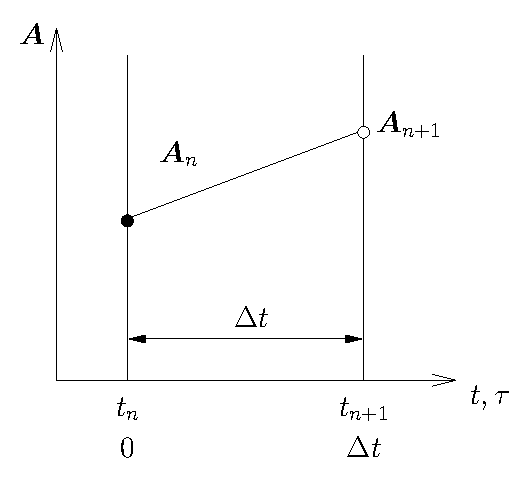
\includegraphics[width=0.32\textwidth]{gfx/lindyn-newmark_acceleration}}
  \subfigure[Velocity]{\label{fig:lindyn-newmark_velocity}
  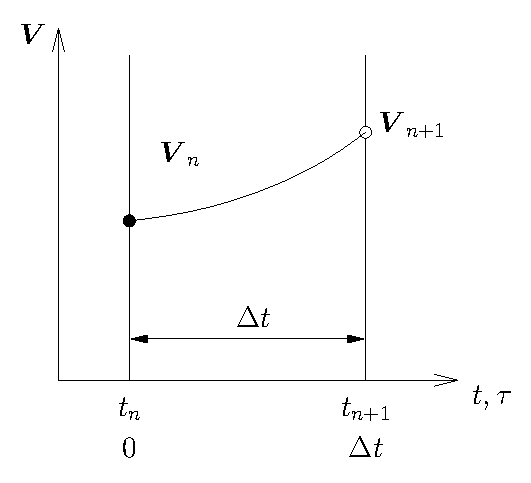
\includegraphics[width=0.32\textwidth]{gfx/lindyn-newmark_velocity}}
  \subfigure[Displacement]{\label{fig:lindyn-newmark_displacement}
  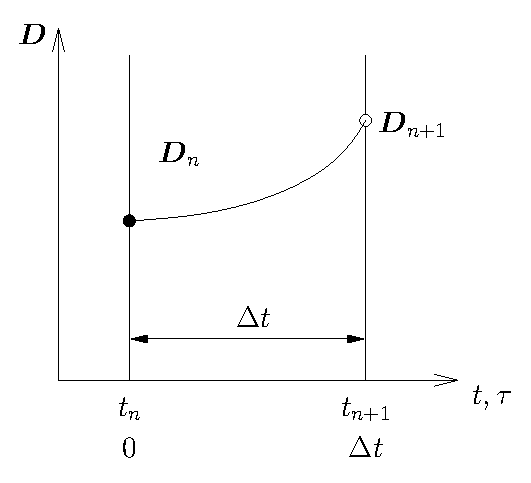
\includegraphics[width=0.32\textwidth]{gfx/lindyn-newmark_displacement}}
  \caption{Newmark scheme approximations}
  \label{fig:lindyn-newmark}
\end{center}
\end{figure}
\begin{equation*}
  \vct{A}(\tau) = \vct{A}_n + \frac{\vct{A}_{n+1} - \vct{A}_n}{\Dt}\tau
\end{equation*}
The integration parameter $\tau$ is defined on the interval $[t_n,t_n+1]$ as $\tau \in[0,\Dt]$.
Now, two parameters are introduced to control the behavior of this approximation
\begin{eqnarray*}
  \vct{A}^\gamma(\tau) &=& \vct{A}_n + 2\gamma \frac{\vct{A}_{n+1} - \vct{A}_n}{\Dt}\tau\\
  \vct{A}^\beta(\tau) &=& \vct{A}_n + 6\beta  \frac{\vct{A}_{n+1} - \vct{A}_n}{\Dt}\tau
\end{eqnarray*}
If \(\gamma=\frac{1}{2}\) and \(\beta=\frac{1}{6}\) are choosen, a linear acceleration scheme is obtaind.
The $\gamma$-parameterized acceleration $\vct{A}^\gamma(\tau)$ is integrated once over $\tau$, which yields
\begin{equation*}
  \vct{V}(\tau) = \vct{A}_n \tau + \frac{2\gamma}{2}\frac{\vct{A}_{n+1} - \vct{A}_n}{\Dt}\tau^2 + c
\end{equation*}
The integration constant $c$ is defined by inserting the known boundary condition of the integral $\vct{V}(\tau=0) = \vct{V}_n$, which gives
\begin{equation*}
  \vct{V}(\tau) = \vct{V}_n + \vct{A}_n \tau + \gamma\frac{\vct{A}_{n+1} - \vct{A}_n}{\Dt}\tau^2\period
\end{equation*}
The new timesteps velocity $\vct{V}_{n+1}$ is therefore obtained at $\vct{V}(\tau = \Dt)$
\begin{equation*}
  \vct{V}_{n+1} = \vct{V}_n + (1-\gamma)\Dt\vct{A}_n  + \gamma\Dt\vct{A}_{n+1}\period
\end{equation*}

Likewise, the $\beta$-parameterized acceleration $\vct{A}^\beta(\tau)$ is integrated to obtain the velocity
\begin{equation*}
  \vct{V}(\tau) = \vct{V}_n + \vct{A}_n \tau + \frac{6\beta}{2}\frac{\vct{A}_{n+1} - \vct{A}_n}{\Dt}\tau^2
\end{equation*}
To obtain the displacement approximation, we integrate again over $\tau$ and yield
\begin{equation*}
  \vct{D}(\tau) = \vct{V}_n \tau + \frac{1}{2}\vct{A}_n \tau^2 + \frac{6\beta}{6}\frac{\vct{A}_{n+1} - \vct{A}_n}{\Dt}\tau^3 + C
\end{equation*}
Inserting the boundary condition $\vct{D}(\tau=0) = \vct{D}_n$, we get the displacement $\vct{D}_{n+1} = \vct{D}(\tau = \Dt)$ at the end of the time interval:
\begin{equation*}
  \vct{D}_{n+1} = \vct{D}_n + \Dt \vct{V}_n  + (\frac{1}{2}-\beta)\Dt^2\vct{A}_n + \beta\Dt^2\vct{A}_{n+1}\period
\end{equation*}

Now we can express the new time steps velocity and acceleration solely from old time steps values and the new displacement as
\begin{eqnarray*}
  \vct{A}_{n+1}
  &=& \frac{1}{\beta\Dt^2} \big( \vct{D}_{n+1} - \vct{D}_n \big)
  - \frac{1}{\beta \Dt} \vct{V}_n
  - \frac{1-2\beta}{2\beta} \vct{A}_n\comma\\
    \vct{V}_{n+1}
  &=& \vct{V}_{n} + \gamma\Dt \vct{A}_{n+1} + (1-\gamma)\Dt\vct{A}_n\period
\end{eqnarray*}

The final pair of equations can be rewritten such that (with $\beta\in[0,\frac{1}{2}]$):
\begin{equation}\label{eq:strdyn:newmark}
\begin{aligned}
& \left\{\begin{array}{rcl}
  \dfrac{\vct{D}_{n+1} - \vct{D}_n}{\Dt}
  & =
  & \vct{V}_n + \frac{\Dt}{2} \big(
    2\beta \vct{A}_{n+1} + (1-2\beta) \vct{A}_n
    \big)
\\
  \dfrac{\vct{V}_{n+1} - \vct{V}_n}{\Dt}
  & =
  & \gamma \vct{A}_{n+1} + (1-\gamma)\vct{A}_n
\end{array}\right.
&& \text{with}
&&\begin{array}{l}
  \beta\in[0,\frac{1}{2}]
\\
  \gamma\in[0,1]
\end{array}
\end{aligned}
\end{equation}
Here, we abbreviated the unknown accelerations at $t_{n+1}$ with with
$\vct{A}_{n+1} = \mat{M}^{-1} \big( -\mat{C} \vct{V}_{n+1} -
\vct{F}_{\Int;n+1} + \vct{F}_{\Ext;n+1}) \big)$. 

This temporal discretisation leads to a
fully discretised set of equations of motion:
\begin{equation}
  \mat{M} \vct{A}_{n+1}
  + \mat{C} \vct{V}_{n+1}
  + \vct{F}_{\Int}(\vct{D}_{n+1})
  = \vct{F}_{\Ext}(t_{n+1})
  \period
\end{equation}

This completely discretised equation of motion is primarily an
$\ndof$-dimensional system of nonlinear equations in the unknown displacements
$\vct{D}_{n+1}$. This statements can be clarified by writing Newmark's method
such that the velocity and acceleration at $t_{n+1}$ are given depending on the
displacements $\vct{D}_{n+1}$:
\begin{align}\label{eq:newmark-velnew}
   \vct{V}_{n+1}(\vct{D}_{n+1})
&  = \frac{\gamma}{\beta\, \Dt} \big( \vct{D}_{n+1} - \vct{D}_n \big)
   - \frac{\gamma-\beta}{\beta} \vct{V}_{n}
   - \frac{\gamma-2\beta}{2\beta}\Dt \vct{A}_n
   \comma
\\ \label{eq:newmark-accnew}
   \vct{A}_{n+1}(\vct{D}_{n+1})
&  = \frac{1}{\beta\, \Dt^2} \big( \vct{D}_{n+1} - \vct{D}_n \big)
   - \frac{1}{\beta\,\Dt} \vct{V}_{n}
   - \frac{1-2\beta}{2\beta} \vct{A}_n
   \period
\end{align}

%%
%%----------------------------
\subsubsection{Generalised-alpha method}
The key idea behind the generalised-alpha method is a modification of the
time point at
which the discretised equations of motion is evaluated. Newmark's method
searches for equilibrium at the end of the current time step $[t_n,t_{n+1}]$,
i.e.\@ at the time $t_{n+1}$. The generalised-alpha method shifts this
evaluation point to  generalised mid-points
$t_{n+1-\alpha_\text{f}}$ and $t_{n+1-\alpha_\text{m}}$, respectively. The non-linear
equation of motion becomes at the generalised mid-point\\
\begin{equation}
  \mat{M} \vct{A}_{n+1-\alpha_\text{m}}
  + \mat{C} \vct{V}_{n+1-\alpha_\text{f}}
  + \vct{F}_{\Int;n+1-\alpha_\text{f}} %%\vct{F}_{\Int}(\vct{D}_{n+1-\alpha_\text{f}})
  = \vct{F}_{\Ext;n+1-\alpha_\text{f}}
\end{equation}

The mid accelerations, velocities, displacements and external forces are
defined as linear combinations of the corresponding start and end vector:\\
\begin{equation}\label{eq:genalpha-middef}
\begin{aligned}
&   \vct{A}_{n+1-\alpha_\text{m}}
    := \big( 1- \alpha_\text{m} \big) \vct{A}_{n+1}
    + \alpha_\text{m} \vct{A}_n
&& \} \quad \alpha_\text{m} \in[0,1]
\\
&   \vct{V}_{n+1-\alpha_\text{f}}
    := \big( 1- \alpha_\text{f} \big) \vct{V}_{n+1}
    + \alpha_\text{f} \vct{V}_n
&&  \multirow{3}{*}{\text{$\Bigg\} \quad \alpha_\text{f} \in[0,1]$}}
\\
&   \vct{D}_{n+1-\alpha_\text{f}}
    := \big( 1- \alpha_\text{f} \big) \vct{D}_{n+1}
    + \alpha_\text{f} \vct{D}_n
&&
\\
&   \vct{F}_{\Ext;n+1-\alpha_\text{f}}
    := \big( 1- \alpha_\text{f} \big) \vct{F}_{\Ext;n+1}
    + \alpha_\text{f} \vct{F}_{\Ext;n}
&&
\end{aligned}
\end{equation}
with the parameters $\alpha_\text{m},\alpha_\text{f}\in[0,1]$. There two possibilties for the internal mid-forces $\vct{F}_{\Int,\text{mid}}$. Either they are defined as well by a linear combination (which we call `TR-like') or by inserting mid-displacements (which we call `IMR-like'), i.e.
\begin{align}
  \text{TR-like} & \quad \vct{F}_{\Int;n+1-\alpha_\text{f}}
    := \big( 1- \alpha_\text{f} \big) \vct{F}_{\Int}(\vct{D}_{n+1})
    + \alpha_\text{f} \vct{F}_{\Int}(\vct{D}_{n})
\\
  \text{IMR-like} & \quad \vct{F}_ {\Int;n+1-\alpha_\text{f}} :=  \vct{F}_{\Int}(\vct{D}_{n+1-\alpha_\text{f}})
\end{align}

The
end-point accelerations and velocities, i.e. $\vct{A}_{n+1}$ and
$\vct{V}_{n+1}$, are related linearly to the end-point displacements
$\vct{D}_{n+1}$ by 
Newmark's method \eqref{eq:newmark-velnew} and
\eqref{eq:newmark-accnew}. Therefore, the mid-equilibrium can be still thought
of a system of nonlinear equations in $\vct{D}_{n+1}$. Let us again write the
unknown mid-velocities and mid-accelerations in terms of $\vct{D}_{n+1}$:
\begin{align}\label{eq:genalpha-velnew}
   \vct{V}_{n+1-\alpha_\text{f}}(\vct{D}_{n+1})
&  = \frac{(1-\alpha_\text{f})\gamma}{\beta\, \Dt} \big( \vct{D}_{n+1} -
     \vct{D}_n \big) 
   - \frac{(1-\alpha_\text{f})\gamma-\beta}{\beta} \vct{V}_{n}
   - \frac{(1-\alpha_\text{f})(\gamma-2\beta)}{2\beta}\Dt \vct{A}_n
   \comma
\\ \label{eq:genalpha-accnew}
   \vct{A}_{n+1-\alpha_\text{m}}(\vct{D}_{n+1})
&  = \frac{1-\alpha_\text{m}}{\beta\, \Dt^2} \big( \vct{D}_{n+1} - \vct{D}_n \big)
   - \frac{1-\alpha_\text{m}}{\beta\,\Dt} \vct{V}_{n}
   - \frac{1-\alpha_\text{m}-2\beta}{2\beta} \vct{A}_n
   \period
\end{align}


The mid-point internal force vector means in terms of assembled element force
vectors:
\begin{equation}
\begin{split}
  \text{TR-like} \quad \vct{F}_{\Int;n+1-\alpha_\text{f}}
&  = \big( 1- \alpha_\text{f} \big) \vct{F}_{\Int;n+1}
    + \alpha_\text{f} \vct{F}_{\Int;n}
\\
&  = \big( 1- \alpha_\text{f} \big) \Ass{e}{\nele} \vct{f}_\Int(\vct{d}_{n+1})
   + \alpha_\text{f} \Ass{e}{\nele} \vct{f}_\Int(\vct{d}_{n})
\\
  \text{IMR-like} \quad \vct{F}_{\Int;n+1-\alpha_\text{f}}
&  = \vct{F}_{\Int}(\vct{D}_{n+1-\alpha_\text{f}})
\\
& = \Ass{e}{\nele} \vct{f}_\Int(\vct{d}_{n+1-\alpha_\text{f}})
  = \Ass{e}{\nele} \int_{\Omega^{(e)}}\limits \left.\big(
  \frac{\pd\vct{E}(\vct{d})}{\pd
  \vct{d}}\big)^\T\right|_{\vct{d}_{n+1-\alpha_\text{f}}}
  \hspace{-2.5em}\vct{S}(\vct{d}_{n+1-\alpha_\text{f}})
  \, \dd V
\end{split}
\end{equation}

\subsubsection{Linearisation and Newton--Raphson iteration}

The generalised mid-point-discretised linear momentum balance can be written
as an residual
\begin{equation}
  \vct{R}_\effdyn(\vct{D}_{n+1})
  = \mat{M} \vct{A}_{n+1-\alpha_\text{m}}
  + \mat{C} \vct{V}_{n+1-\alpha_\text{f}}
  + \vct{F}_{\Int;n+1-\alpha_\text{f}}
  - \vct{F}_{\Ext;n+1-\alpha_\text{f}}
  \stackrel{!}{=} \vct{0}
\end{equation}
These nonlinear equations can be linearised at the end of the time step at
$t_{n+1}$ with $\vct{D}_{n+1}$: 
\begin{equation}
  \Lin\vct{R}_\effdyn(\vct{D}_{n+1})
  = \vct{R}_\effdyn(\vct{D}_{n+1}^i) 
  + \left.\frac{\pd \vct{R}_\effdyn(\vct{D}_{n+1})}
    {\pd \vct{D}_{n+1}}\right|^{i}  \Delta\vct{D}_{n+1}^{i+1}
\end{equation}
in which the \intro{dynamic effective tangential stiffness matrix}
$\mat{K}_{\Tang\,\effdyn}$ appears as the differentiation of the dynamic
effective residual with respect to the displacements $\vct{D}_{n+1}$. This
stiffness matrix is obtained detailed in\\
\begin{equation}
\begin{aligned}
&  \mat{K}_{\Tang\,\effdyn}(\vct{D}_{n+1}^i)
   = \left.\frac{\pd \vct{R}(\vct{D}_{n+1})}{\pd \vct{D}_{n+1}}\right|^{i}
\\
& 
  \quad = \Bigg.\Bigg[\mat{M} 
          \underbrace{\frac{\pd \vct{A}_{n+1-\alpha_\text{m}}}{\pd \vct{A}_{n+1}}}_{1-\alpha_\text{m}}
          \underbrace{\frac{\pd\vct{A}_{n+1}}{\pd\vct{D}_{n+1}}}_{\frac{1}{\beta\Dt^2}}
   +     \vct{C}
          \underbrace{\frac{\pd \vct{V}_{n+1-\alpha_\text{f}}}{\pd \vct{V}_{n+1}}}_{1-\alpha_\text{f}}
          \underbrace{\frac{\pd\vct{V}_{n+1}}{\pd\vct{D}_{n+1}}}_{\frac{\gamma}{\beta\Dt}}
   +     \frac{\pd\vct{F}_{\Int,n+1-\alpha_\text{f}}}{\pd\vct{D}_{n+1}}
    \Bigg]\Bigg|^i
\\
&  \quad = \Bigg.\Bigg[
   \frac{1-\alpha_\text{m}}{\beta \Dt^2} \mat{M}
   + \frac{(1-\alpha_\text{f})\gamma}{\beta\Dt} \mat{C}
   + \frac{\pd\vct{F}_{\Int,n+1-\alpha_\text{f}}}{\pd\vct{D}_{n+1}}
   \Bigg]\Bigg|^i
\end{aligned}
\end{equation}
with
\begin{align}
   \text{TR-like} & \quad \frac{\pd\vct{F}_{\Int,n+1-\alpha_\text{f}}}{\pd\vct{D}_{n+1}}
   = \frac{\pd\vct{F}_{\Int}(\vct{D}_{n+1-\alpha_\text{f}})}{\pd\vct{D}_{n+1-\alpha_\text{f}}} 
   \frac{\pd\vct{D}_{n+1-\alpha_\text{f}}}{\pd\vct{D}_{n+1}}
   = \big( 1-\alpha_\text{f} \big)  \mat{K}_\Tang(\vct{D}_{n+1-\alpha_\text{f}})
\\
   \text{IMR-like} & \quad \begin{array}{ll} \frac{\pd\vct{F}_{\Int,n+1-\alpha_\text{f}}}{\pd\vct{D}_{n+1}}
   & = \frac{\pd}{\pd\vct{D}_{n+1}} \Big( \big( 1- \alpha_\text{f} \big) \vct{F}_{\Int}(\vct{D}_{n+1})
    + \alpha_\text{f} \vct{F}_{\Int}(\vct{D}_{n}) \Big) \\
   & = \big( 1-\alpha_\text{f} \big)  \frac{\pd\vct{F}_{\Int}(\vct{D}_{n+1})}{\pd\vct{D}_{n+1}}
   = \big( 1-\alpha_\text{f} \big) \mat{K}_\Tang(\vct{D}_{n+1})
   \end{array}
\end{align}

In a Newton--Raphson iteration the iterative displacement increment
$\incr\vct{D}_{n+1}^{i+1}$ is calculated by solving
\begin{align}
&  \mat{K}_{\Tang\,\effdyn}(\vct{D}_{n+1}^i)\, \Delta\vct{D}_{n+1}^{i+1}
  = - \vct{R}_\effdyn(\vct{D}_{n+1}^i)
\\
& \qquad\qquad\qquad\leadsto\qquad
  \Delta\vct{D}_{n+1}^{i+1}
  = - {\mat{K}_{\Tang\,\effdyn}(\vct{D}_{n+1}^i)}^{-1} \vct{R}_\effdyn(\vct{D}_{n+1}^i)
\end{align}

This allows to update the unknown displacements with
\begin{equation}
  \vct{D}_{n+1}^{i+1}
  = \vct{D}_{n+1}^{i} + \Delta\vct{D}_{n+1}^{i+1}
  \period
\end{equation}
In essence, the actual right-hand-side $\vct{R}_\effdyn(\vct{D}_{n+1}^{i})$ depends as shown only on the actual end-displacements $\vct{D}_{n+1}^{i+1}$,
but it is convenient to calculate $\vct{R}_\effdyn(\vct{D}_{n+1}^i)$ using
the 
current mid-displacements, -velocities and -accelerations. These
current vectors can be calculated based on the formulas given in
\eqref{eq:genalpha-middef} or \eqref{eq:genalpha-velnew} and
\eqref{eq:genalpha-accnew}.  Optionally, they can be evaluated with an update
mechanism with these increments
\begin{equation}
\begin{aligned}
   \Delta\vct{D}_{n+1-\alpha_\text{f}}^{i+1}
&   = \frac{\pd\vct{D}_{n+1-\alpha_\text{f}}}{\pd\vct{D}_{n+1}} 
     \, \Delta\vct{D}_{n+1}^{i+1}
   = (1-\alpha_\text{f}) \, \Delta\vct{D}_{n+1}^{i+1}
\\
   \Delta\vct{V}_{n+1-\alpha_\text{f}}^{i+1}
&   = \frac{\pd\vct{V}_{n+1-\alpha_\text{f}}}{\pd\vct{D}_{n+1}} 
     \, \Delta\vct{D}_{n+1}^{i+1}
   = \frac{(1-\alpha_\text{f})\gamma}{\beta \Dt} \, \Delta\vct{D}_{n+1}^{i+1}
\\
   \Delta\vct{A}_{n+1-\alpha_\text{m}}^{i+1}
&   = \frac{\pd\vct{A}_{n+1-\alpha_\text{m}}}{\pd\vct{D}_{n+1}} 
     \, \Delta\vct{D}_{n+1}^{i+1}
   = \frac{1-\alpha_\text{m}}{\beta \Dt^2} \, \Delta\vct{D}_{n+1}^{i+1}
\end{aligned}
\end{equation}
and the usual update procedure
\begin{equation}
\begin{aligned}
   \vct{D}_{n+1-\alpha_\text{f}}^{i+1}
&  = \vct{D}_{n+1-\alpha_\text{f}}^{i} 
   + \Delta\vct{D}_{n+1-\alpha_\text{f}}^{i+1}
\\
   \vct{V}_{n+1-\alpha_\text{f}}^{i+1}
&  = \vct{V}_{n+1-\alpha_\text{f}}^{i} 
   + \Delta\vct{V}_{n+1-\alpha_\text{f}}^{i+1}
\\
   \vct{A}_{n+1-\alpha_\text{m}}^{i+1}
&  = \vct{A}_{n+1-\alpha_\text{m}}^{i} 
   + \Delta\vct{A}_{n+1-\alpha_\text{m}}^{i+1}
\\
\end{aligned}
\end{equation}

The convergence of the Newton--Raphson iteration can be tested --- for
instance --- by checking the residual
\begin{equation}
  \Abs{ \vct{R}_\effdyn(\vct{D}_{n+1}^{i+1}) } \leq \tol
  \period
\end{equation}
A different relative convergence check  is based on the  displacement
increment:
\begin{equation}
  \frac{\Abs{ \Delta\vct{D}_{n+1}^{i+1} }}
  {\Abs{ \vct{D}_{n+1}^{i+1} - \vct{D}_n }} 
  \leq \tol_\text{D}
  \period
\end{equation}


\subpart{Algorithm Newton--Raphson iteration}\\

\begin{struktogramm}(145,100)
\assign{Read initial time / conditions: $t_0$, $\vct{D}_0$, $\vct{V}_0$}
\assign{Generate mass and damping matrix: $\mat{M}$ and $\mat{C}$}
\assign{Calculate initial accelerations: $\vct{A}_0 = \mat{M}^{-1}
  \big(-\mat{C}\vct{V}_0 - \vct{F}_{\Int}(\vct{D}_0) +
  \vct{F}_{\Ext}(t_0)\big)$}
\while{Time loop over time steps $n=0,1,\ldots$ while  $t_n\leq t_E$}
   \assign{Predictor (simple): $\vct{D}_{n+1}^{i=0} := \vct{D}_n$
      $\leadsto$ $\vct{D}_{n+1-\alpha_\text{f}}^{i=0}$,
      $\vct{V}_{n+1-\alpha_\text{f}}^{i=0}$,
      $\vct{A}_{n+1-\alpha_\text{m}}^{i=0}$}
   \assign{Load vector: $\vct{F}_{\Ext;n+1-\alpha_\text{f}}$}
   \assign{Residual: $\vct{R}_\effdyn(\vct{D}_{n+1}^{i=0})$}
   \while{Newton loop $i=0,1,\ldots$  while $\Abs{
       \vct{R}_\effdyn(\vct{D}_{n+1}^{i}) } > \tol$}
      \assign{Generate effective dynamic stiffness matrix:
        $\mat{K}_{\Tang\,\effdyn}^i$}
      \assign{Solve displ. iter. incr.: 
        $\mat{K}_{\Tang\,\effdyn}^i \, \Delta\vct{D}_{n+1}^{i+1}
        = - \vct{R}_\effdyn(\vct{D}_{n+1}^{i})$
%        $\leadsto$
%        $\Delta\vct{D}_{n+1}^{i+1}$
        }
      \assign{Update displacements: $\vct{D}_{n+1}^{i+1} := \vct{D}_{n+1}^i +
        \Delta\vct{D}_{n+1}^{i+1}$}
      \assign{Update mid-displ., -vel., -acc.: 
        $\vct{D}_{n+1-\alpha_\text{f}}^{i+1}$,
        $\vct{V}_{n+1-\alpha_\text{f}}^{i+1}$,
        $\vct{A}_{n+1-\alpha_\text{m}}^{i+1}$}
      \assign{Generate effective dynamic residual: $\vct{R}_\effdyn^{i+1}$}
     \assign{Update iteration counter: $i := i + 1$}
   \whileend
   \assign{Update time step: $n := n+1$}
   \assign{Update time: $t_{n+1} := t_n + \Dt$}
\whileend
\end{struktogramm}

Here we have used a very simple predictor for the new displacements (and in
consequence for velocities and accelerations): The previously converged time
step is used.  More sophisticated
predictors can be constructed introducing extrapolation techniques or
explicit time integration schemes. For instance, the forward
Euler time integration scheme could be applied as a predictor (forward Euler
was introduced in the course ``Finite Elemente''); however, forward Euler is
not a recommended choice.

\subsubsection{Order of accuracy}
According to Section \ref{strdyn:sec:accuracy} we can deduce the order of accuracy of the displacement approximation given by the generalised-alpha (GA) method. We achieve
\begin{align}
   \vct{l}_{n+1}^{\text{GA}}
&  = \vct{D}(t_{n+1}) - \vct{\Psi}_{n+1,n}^{\text{GA}} \vct{D}(t_n)
\\
&  = \dt^3 \Big( \frac{1}{6} - \frac{1-\alpha_\text{f}}{1-\alpha_\text{m}} \beta \Big) 
   \dotvct{A}(t_n)
   + \dt^4 \Big( \frac{1}{6} - \frac{1-\alpha_\text{f}}{1-\alpha_\text{m}} \beta \Big)  
   \ddotvct{A}(t_n) 
   + \OO(\dt^5)
\end{align}
This equation implies: The displacements are always at least $2$nd order accurate and they are even $3$rd order accurate if $\frac{1}{6} - \frac{1-\alpha_\text{f}}{1-\alpha_\text{m}} \beta = 0$. 

Since the governing equations are a set of second order ODEs, we provide the LDE of the velocities as well. These are
\begin{align}
   \dotvct{l}_{n+1}^{\text{GA}}
&  = \vct{V}(t_{n+1}) - \dotvct{\Psi}_{n+1,n}^{\text{GA}} \vct{V}(t_n)
\\
&  = \dt^2 \Big( \frac{1}{2} - \frac{1-\alpha_\text{f}}{1-\alpha_\text{m}} \gamma \Big) 
   \dotvct{A}(t_n)
   + \dt^3 \Big( \frac{1}{6} - \frac{1-\alpha_\text{f}}{1-\alpha_\text{m}} \gamma \Big)  
   \ddotvct{A}(t_n) 
   + \OO(\dt^4)
\end{align}
in which $\dotvct{l}_{n+1}^{\text{GA}}$ and $\dotvct{\Psi}_{n+1,n}^{\text{GA}}$ do \emph{not} imply a time differentation -- the dot is merely a notation. It can be seen the velocities are $2$nd order accurate if $\frac{1}{2} - \frac{1-\alpha_\text{f}}{1-\alpha_\text{m}} \gamma$ otherwise only $1$st order.

As stated before, the semi-discrete equations of motion are second order ODE, thus both LDEs have to be taken into account and the worse value determines the overall order of accuracy according to \name{Hairer} \etal{} \cite{hairer87, hairer91}). 

\subsection{Shortcomings in \ccarat{} implementation}
Individual/No load curves. Currently, all external loads are scaled with
  the load curve \kw{CURVE1}, which \emph{must} be applied


%%
%%............................generalised energy-momentum-conserving
\section{Generalized energy-momentum method -- \ccarat{} Gen\_EMM}
Coded by Izzet \"{O}zdemir (Master thesis ``An approach to contact in
computational structural dynamics'', 2003)

The routine
\begin{enumerate}
\item is supposed for
  \begin{itemize}
  \item WALL1
  \item SHELL8 is malware $\to$ remove
  \end{itemize}
\item is based on Simo \& Tarnow energy-momemtum conserving scheme, giving
  an asymmetric stiffness matrix 
\item conserves total energy -- Tested with
  prescribed boundary displacement, loads were not applied.
\item conserves total energy, linear and angular momemtum. Tested with
  unsupported body, loads are switched off with 1st Load Curve after a while. 
\item does not extract external (potential) loads, bad to test for
  conservative loading 
\item Contact was not tested (node-to-segment)
\item possesses adaptive time-step fragments
\item src/Input \cod{w1\_gemm\_contact\_emconserv.dat}
\end{enumerate}

\subitempart{Suggestions}
\begin{enumerate}
\item Check thoroughly
\item Improve on WALL1 calculation; right now activation is controlled by
  pre-proccessor flag such that either generalised-$alpha$ or GEMM is
  available; maybe new ACTION, or flag in wall1(...)
\item Add SOLID3
\end{enumerate}

%%
%%............................central differences
\section{Central differences -- \ccarat Centr\_Diff}
Algorithm:
\begin{gather*}
  \left\{\begin{array}{l}
     \vct{D}_{n+1} = \vct{D}_n + \Dt \vct{V}_n + \frac{\Dt^2}{2} \vct{A}_n
  \\
     \vct{A}_{n+1} = \mat{M}^{-1} \big( 
                     \vct{F}_\Int(\vct{D}_{n+1}) 
                     - \vct{F}_\Ext(t_{n+1})
                     \big)
  \\
     \vct{V}_{n+1} 
               = \vct{V}_n + \frac{\Dt}{2} \big( 
               \vct{A}_n + \vct{A}_{n+1} \big)
  \end{array}\right.
\end{gather*}
\begin{enumerate}
\item Method works explicitly for a few elements. Un-/Supported elements
  \begin{itemize}
  \item[$+$] WALL1, SHELL8, SHELL9
  \item[$-$] BRICK1, BEAM3, WALLGE
  \end{itemize}
\item src/Input \cod{krag\_2ele\_expl.dat}
\end{enumerate}

\subitempart{Suggestions}
\begin{enumerate}
\item Add time step-size adapitvity
\item Store inverted mass matrix once and for all; or even dummy solver for
  lumped mass matrix
\end{enumerate}

%%
%%............................Adaptivity
\section{Time adaptivity}

\subsection{Theory of time adaptivity based on indication of the local discretisation error}
Different ways exist to adapt the time step size $\Dt$, here we only apply an \lat{a posteriori} method utilising the local discretisation error (LDE). 



\subsubsection{Step size adaptivity} \label{sec:adaptivity}
Local error control is based on requiring the estimated local
discretisation error to stay below a user-defined tolerance
$\tol$\@. If the local discretisation error, resulting from a time integration with time
step size $\Delta t_n$, is higher than the tolerance, the step is
repeated with a smaller step size. A proposal for this smaller step size is the so-called `optimal' step size, denoted with $\dt_n^*$, which
is the time step size resulting in a local discretisation error which is approximately equal to the
tolerance. The procedure is repeated until a small enough step size is
found. Then the `optimal' time step size might be used as an initial value
for the next time step size $\Delta t_{n+1} = \Delta t_n^*$\@. 

Therefore the basic requirement for the local discretisation error is
\begin{equation} \label{eq:lde-leq-tol}
  \Abs{\vct{l}_{n+1}(\dt_n)} \leq \tol
%%  \comma\quad \tol > 0
  \comma
\end{equation}
whereby the dimensionless tolerance $\tol>0$ is user-prescribed. The above
described procedure is contained in 
Figure~\ref{fig:adap-sch}\@. 
\begin{figure}[ht!]
\begin{center}
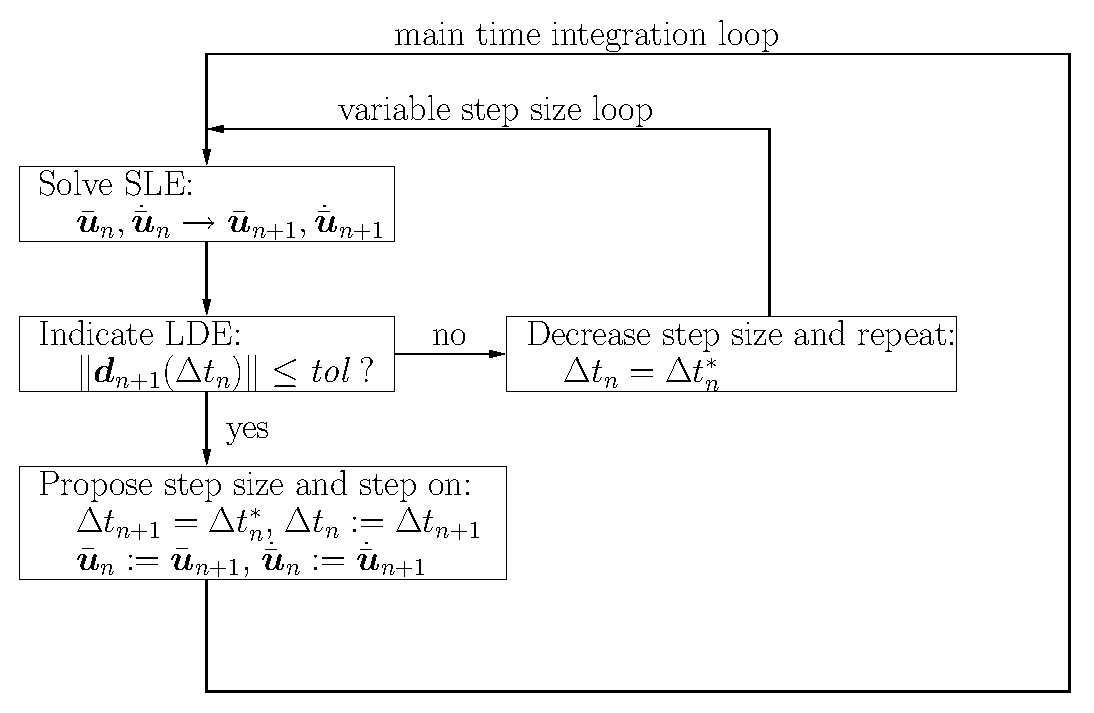
\includegraphics[width=0.6\textwidth]{gfx/adap-sch}
\caption{Diagram of LDE-based step size adaptivity}
\label{fig:adap-sch}
\end{center}
\end{figure}
Different norms, such as 
average, root-mean-square or infinity norm, can be used to obtain a
dimensionless scalar from the local discretisation error vector
(Appendix~\ref{app:norms})\@. 

The `optimal' step size
$\Delta t_n^*$ is derived in the following equations. The starting point is
the usual definition of the local discretisation error in which the local discretisation error obtained with $\dt_n$ is
assumed to be larger than $\tol$:
\begin{gather}
  \label{LDE-old-step-size-greater-tol}
  \Abs{ \vct{l}_{n+1}(\Delta t_n) }
  \approx \vct{C}(t_n)\, \Delta t_n^{p+1} 
  \geq \tol
  \comma
\\
  \label{LDE-new-step-size-approx-tol}
  \Abs{ \vct{l}_{n+1}(\Delta t_n^*) }
  \approx \vct{C}(t_n)\, {\Delta t_n^*}^{p+1} 
  \approx \tol
  \period
\end{gather}
Equation \eqref{LDE-new-step-size-approx-tol} can be transformed to
\begin{equation} \label{LDE-new-step-size-approx-tol-2}
  \vct{C}(t_n)
  \approx \frac{\Abs{ \vct{l}_{n+1}(\Delta t_n^*) }}{{\Delta
  t_n^*}^{p+1}}
  \approx \frac{\tol}{{\Delta t_n^*}^{p+1}}
  \period
\end{equation}

Introducing (\ref{LDE-new-step-size-approx-tol-2}) into
(\ref{LDE-old-step-size-greater-tol}) results in
\begin{equation}\label{new-step-size}
  \Delta t_n^* \leq \sqrt[{p+1}]{\frac{\tol}{\Abs{
  \vct{l}_{n+1}(\Delta t_n) }}}\, \Delta t_n
  \period
\end{equation}
The `optimal' step size corresponds to the lower bound in
\eqref{new-step-size}\@. 

Furthermore, the `optimal' step size might be more reliable if the
tolerance is reduced by `safety' scale factors
\begin{equation}\label{eq:new-step-size-scaled}
  \dt_n^\text{new}
  = \min\big\{ \dt_\text{max}, \max\{\min\big( r_\text{max}, \max(
  r_\text{min}, s r^*)\dt_n, \dt_\text{min} \} \big\}
  \period
\end{equation}
In the previous equation the `optimal' ratio is abbreviated with
\begin{equation}\label{eq:new-step-size-optscal}
  r^* = \sqrt[{p+1}]{\frac{\tol}{\Abs{
  \vct{l}_{n+1}(\Delta t_n) }}}
  \period
\end{equation}
The step size $\dt_n^\text{new}$,  \eqref{eq:new-step-size-scaled},
replaces the `optimal' step size $\dt_n^*$ in 
the algorithm (Figure \ref{fig:adap-sch})\@. The factor $r_\text{max}$
limits the maximum size increase between two steps, $r_\text{min}$ bounds the
decrease. 
In the same spirit, a
maximum and minimum step size, $\dt_\text{max}$ and $\dt_\text{min}$, is
imposed to achieve a more robust algorithm. Sometimes, $p$ instead of $(p+1)$
is 
used in \eqref{eq:new-step-size-optscal} to reflect the order of the
global error. 
\newline

Generally speaking, estimations for the local discretisation error are
obtained by using two different time integration schemes A and B\@. 
The
comparison of results $\vct{y}_{n+1}^\text{A}$ to
$\vct{y}_{n+1}^\text{B}$ makes it possible to evaluate an local discretisation error estimation of
the lower-order method of scheme A or B\@. If
the results of the scheme A are kept to integrate forward 
in time, then A is called \intro{marching} time integration scheme. The scheme
B is only used to indicate the local discretisation error, hence it is referred to as
\intro{auxiliary} scheme. The adaptive algorithm is denoted with B/A\@. 

The algorithms based on 
embedded \name{Runge}-\name{Kutta} methods are instances of such local error
control with time step adaption.

\subsection{\name{Zienkiewicz} and \name{Xie} indicator}\label{sec:zx}
\name{Zienkiewicz} and \name{Xie} presented in \cite{zienkiewicz91} a local
error indicator for the \name{Newmark} algorithm (Section
\ref{sec:new})\@. The estimator advantageously uses the member which
integrates the displacements with third-order accuracy, \ie{}
$\beta=\frac{1}{6}$, $\gamma$ arbitrary, \cf{} \eqref{eq:new-lde-1}\@. The concept can be straight forwardly applied to the generalised-alpha method.

In essence, the general generalised-alpha method with $2$nd order accurate displacements (dubbed here GA2 with $\beta\neq\frac{1}{6}\cdot\frac{1-\alpha_\text{m}}{1-\alpha_\text{f}}$) is considered as the marching time integration scheme. Its $3$rd order accurate sibling GA3 is used as the auxiliary scheme to eventually obtain the
local discretisation error estimation/indication of the displacements. 

The GA2 and GA3 methods are implicit schemes, hence a
direct calculation with GA2 and GA3 would require two
iterative solutions. This can be overcome by avoiding a direct determination
of the GA3\@.
The results of the marching GA2 method ($\vct{D}_{n+1}^\text{GA2}$,
$\vct{V}_{n+1}^\text{GA2}$, $\vct{A}_{n+1}^\text{GA2}$) can be used
to explicitely construct a third-order accurate result, which is related to
the NM3 and is called ZX here\@. 

The ZX method is defined as
\begin{equation*}
  \vct{D}_{n+1}^\text{ZX}
  = \vct{D}_n + \dt_n \vct{V}_n + \frac{\dt^2}{3}\vct{A}_n
  + \frac{\dt^2}{6} \vct{A}_{n+1}^\text{GA2}
  \period
\end{equation*}
The dependence of this algorithm on $\vct{D}_{n+1}^\text{GA2}$ is revealed
by introducing \eqref{eq:new-algo}
\begin{equation}\label{eq:zx-algo}
  \vct{D}_{n+1}^\text{ZX}
  = \frac{1}{6\beta} \Big( \vct{D}_{n+1}^\text{GA2}
  + (6\beta-1)(\vct{D}_n + \dt\vct{V}_n +
  \frac{\dt^2}{2}\vct{A}_n) \Big)
  \quad\text{with}\quad
  \beta\neq\frac{1}{6}
  \period
\end{equation}
The local discretisation error of the ZX is based on \eqref{eq:zx-algo} by expanding it in
\name{Taylor} series:
\begin{equation*}
  \vct{l}_{n+1}^\text{ZX}
  = \vct{D}(t_{n+1}) - \mat{\Psi}_{n+1,n}^\text{ZX}\vct{D}(t_n) 
  = -\frac{\dt^4}{24} \barmat{u}^{(4)}(t_n) + \OO(\dt^5)
  \comma
\end{equation*}
in which the third-order accuracy is shown.

\name{Zienkiewicz} and \name{Xie}'s indicator of the local discretisation error uses the
definitions of the local discretisation errors for the displacements and assumes direct differences
as feasible approximations
\begin{subequations}
\begin{equation}\label{eq:zx-nm-lde1}
  \vct{l}_{n+1}^\text{GA2}
  = \vct{D}(t_{n+1}) - \mat{\Psi}_{n+1,n}^\text{GA2}\vct{D}(t_n) 
  \approx \vct{D}(t_{n+1}) - \vct{D}_{n+1}^\text{GA2}
  = \OO(\dt^3)
  \comma
\end{equation}
\begin{equation}\label{eq:zx-nm-lde2}
  \vct{l}_{n+1}^\text{ZX}
  = \vct{D}(t_{n+1}) - \mat{\Psi}_{n+1,n}^\text{ZX}
  \approx \vct{D}(t_{n+1}) - \vct{D}_{n+1}^\text{ZX}
  = \OO(\dt^4)
  \period
\end{equation}
\end{subequations}
Equations \eqref{eq:zx-nm-lde1} and
\eqref{eq:zx-nm-lde2} are subtracted from each other leading to
\begin{equation*}
  \vct{l}_{n+1}^\text{GA2}
  = \vct{D}_{n+1}^\text{ZX} -\vct{D}_{n+1}^\text{GA2}
  \comma
\end{equation*}
as $\vct{l}_{n+1}^\text{ZX}$ is negligible compared to
$\vct{l}_{n+1}^\text{GA2}$\@. The indicator is given alternatively as
\begin{equation*}
  \vct{l}_{n+1}^\text{GA2}
  = \frac{\dt^2}{6} ( 1 - 6\beta )
  \big( \vct{A}_{n+1}^\text{GA2} -\vct{A}_{n} \big)
  \comma
\end{equation*}
which coincides with the formula of \name{Zienkiewicz} and \name{Xie}
\cite{zienkiewicz91} except the sign.

The presented local discretisation error estimator allows only to assess the
displacements, the velocities are not checked. 


%%
%%............................Inclined BCs for retro-discretisation
\section{Inclined boundary conditions (BCs) -- \ccarat{}}

\subsection{About}
Sometimes it is desirable to have boundary conditions
which are not oriented in the global Cartesian $XYZ$-axes,
but in other directions. This occurs for instance with
rotatory symmetric problems.

\subsection{Method}
The implementation is an adaptation of Steffen Genkinger's
local systems (locsys, for fluid) to structures.
The idea is to rotate the DOFs on an inclined boundary in the
direction of a local co-ordinate system. These locally oriented
DOFs are solved on the global level. The generalised-alpha holds
locally oriented DOFs for all DOFs at Dirichlet nodes
(prescribed/supported \& free DOFs there). Therefore, all assembled
quantities (stiffness, mass, internal force, velocity, etc) have
at certain nodes rotated DOFs. On the other hand, the `\texttt{sol}', 
`\texttt{sol\_increment}', etc arrays at the \texttt{NODE}s are always globally
oriented (except for intermediate operations at solution algo level)

\subsection{Gid input}
\begin{enumerate}
\item Define \& name (e.g. `\textit{mysys}') local axes\\
       Data $\to$ Local axes $\to$ Define
\item Assign local systems to design points, lines and surface to which
       inclinded BCs are wanted. E.g.\\
       \texttt{Data} $\to$ \texttt{Conditions} $\to$ \texttt{Single} $\to$ \texttt{Layer} $\to$ \texttt{Points} $\to$ \texttt{Locsys Point}\\
       choose \texttt{LocsysId} (e.g. \textit{1})\\
       You need to apply to the full hierarchy
       of design element. It avoids conflicts on lines which belong
       to different Dirichlet BCs coming from higher entities.
\item Bind to \texttt{locsysId} the named  (e.g. `\textit{mysys}') local axes\\
       Data $\to$ Problem Data $\to$ Locsys\\
       \texttt{Locsys\_1} : \texttt{on}\\
       \texttt{Locsys\_Typ\_1} : \texttt{BASEVEC}\\
       \texttt{Ls1\_Basevec\_Input\_Type} : \texttt{LocalAxes\_Name}\\
       \texttt{Ls1\_LocalAxes\_Name} : `\textit{mysys}'\\
\end{enumerate}

\subsection{Compilation}
\texttt{LOCALSYSTEMS\_ST} preprocessor definition required (\texttt{defines} file)

\subsection{Restrictions}
\begin{itemize}
\item Available in old discretisation
\item Implemented for 
   \begin{itemize}
   \item \texttt{WALL1} (untested)
   \item \texttt{BRICK1} (untested)
   \item \texttt{SOLID3} (verified)
   \end{itemize}
\item Prescribed deflection of DOFs available
\item Solution technique: Generalised-alpha (\texttt{stru\_dyn\_nln.c})
\item fsiloads in \texttt{WALL1}???
\item test file \texttt{so3\_dyn\_inclined\_bc.dat}
\end{itemize}